% !TeX spellcheck = ru_RU
\chapter{Сопровождение людей в видеопоследовательности} \label{chapt5}


Предлагаемый алгоритм состоит из четырех этапов:
\begin{enumerate}
	\item поиск людей на кадрах видеопоследовательности;
	\item построение треклетов;
	\item построение траекторий сопровождаемых людей;
	\item восстановление положения людей на кадрах видеопоследовательности, где они не были обнаружены (рисунок 1).
\end{enumerate}

В следующих пунктах эти шаги будут рассмотрены подробнее.

Обнаружение людей

Для поиска людей на кадрах видеопоследовательности используется детектор голов людей \cite{prisacariu_reid_tr2310_09}. Он возвращает множество прямоугольников, ограничивающих изображение голов людей. Это позволяет находить людей, часть изображения которых перекрыта. Такая ситуация часто возникает в кадрах с большим количеством людей в ней. Так как камеры видеонаблюдения обычно снимают сцену сверху, то головы большинства людей, присутствующих в ней, видны в
кадре.

Обычно среди обнаружений детектора есть несколько ложных срабатываний. Размеры многих из них не соответствуют размерам головы человека, характерным для данной области
изображения. Поэтому предлагается проводить фильтрацию обнаружений по размерам. В предлагаемом алгоритме вычисляется размер каждого обнаружения в мировой системе координат, и используются пороговые значения для разделения ложных срабатываний детектора и верно обнаруженных голов людей. Благодаря фильтрации по размеру обнаружений в мировой системе координат, используемые пороговые значения не зависят от положения найденной области на изображении. В алгоритме используется предположение о постоянстве отношения роста человека к размеру его головы. Описанное предположение и матрица калибровки камеры позволяют определить положение человека на плоскости земли и размер его головы в мировой системе координат.

Построение треклетов.

Для каждого обнаруженного изображения головы строится треклет, объединяющий информацию о положении обнаружения и оценки скорости человека в 3небольшой временной окрестности кадра, где он был обнаружен. Для построения оценок скорости на соседних кадрах видеопоследовательности в статье \cite{benfold2011stable} предлагается использовать сопровождение нескольких уголков \cite{shi1994good} изображения головы человека алгоритмом KLT~\cite{tomasi1991detection}. Так же авторы~\cite{benfold2011stable} предлагают проводить сопровождение уголков не только в прямом направлении, но и в обратном, то есть в направлении убывания номера кадра. Для построения каждой оценки скорости используется положение головы человека на кадре, где он был обнаружен, и его положение, определенное алгоритмом визуального сопровождения. Полученные оценки имеют большое значение при построении траекторий.

Наши эксперименты показали, что алгоритм KLT является недостаточно надежным для получения качественных оценок скорости сопровождаемых людей. Алгоритм неверно определяет положение большого количества сопровождаемых уголков изображения (рисунок~\ref{sec::tracking::fig::visual_tracking}). Поэтому для построения более надежных скорости предлагается использовать алгоритм «Стая точек»~\cite{kolsch2004fast}. Данный алгоритм определяет положение человека в кадре, сопровождая несколько уголков его изображения. В отличие от KLT алгоритм «Стая точек» позволяет обнаруживать и повторно инициализировать уголки, положение которых было неверно определено на текущем кадре. Так же, когда изображение головы слабо текстурировано, на нем не удается найти достаточное количество уголков, которые можно было бы надежно сопровождать алгоритмами KLT и «Стая точек». Это происходит, когда изображение головы имеет небольшие размеры, или человек повернут спиной к камере. В таких ситуациях сопровождение алгоритмом на основе кросс-корреляции шаблонов~\cite{freeman1998computer} дает более надежные оценки скорости.

Построение траекторий

На этом шаге решается задача разбиения множества треклетов $D$, относящихся к кадрам скользящего окна, на траектории сопровождаемых людей. Траекторией называется множество всех треклетов, отнесенных к обнаружениям одного человека. Из определения следует, что траектория не может содержать несколько треклетов, относящихся к одному и тому же кадру видеопоследовательности. Более того каждый треклет может принадлежать лишь одной траектории. Любое множество траекторий $\left\{T_j\right\}$, удовлетворяющее указанным ограничениям, будем называть гипотезой $H$. Таким образом, задача построения траекторий является задачей нахождения оптимальной гипотезы $H^*$.

Для описанной задачи вводится вероятностное пространство на множестве допустимых гипотез таким образом, что наиболее вероятная гипотеза представляет лучшее разбиение множества треклетов на траектории:
\begin{equation}
	H^* = \argmax_H P(H|D) = \argmax_H P(H, D)
	\label{sec::tracking::opt_hyp}
\end{equation}

\begin{figure}[t]
	\begin{center}
		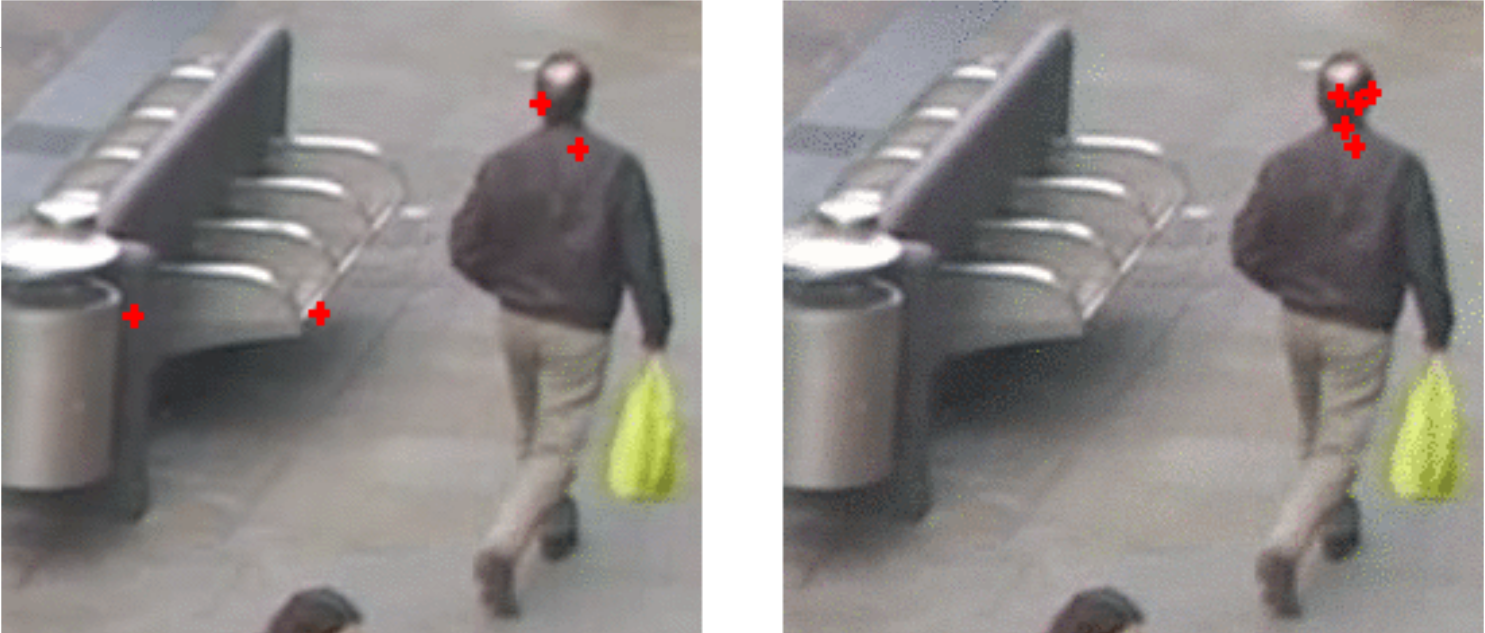
\includegraphics[width=150mm]{tracking/visual_tracking}
		\caption{Положения уголков (отмечены красными крестами), полученные при сопровождении в течение 75 кадров алгоритмом KLT (слева) и алгоритмом <<Стая точек>> (справа).}
		\label{sec::tracking::fig::visual_tracking}
	\end{center}
\end{figure}

Таким образом, для описания алгоритма построения траекторий требуется:
\begin{itemize}
	\item Задать вероятностное пространство через описание модели движения;
	\item Определить метод поиска оптимальной гипотезы.
\end{itemize}

\begin{figure}[t]
	\begin{center}
		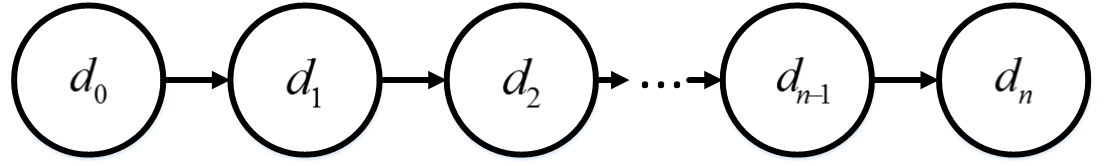
\includegraphics[width=150mm]{tracking/MarkovChain}
		\caption{Графическая модель траектории движения человека. ${d_i}$ "--- множество треклетов рассматриваемой траектории.}
		\label{sec::tracking::fig::markov_chain}
	\end{center}
\end{figure}

Модель движения

Для упрощения модели можно предположить, что люди в сцене движутся независимо друг от друга, то есть треклеты, относящиеся к разным траекториям независимы. Таким образом, модель движения людей предлагается представить в виде независимого множества траекторий.

В настоящей работе траектория движения человека моделируется динамической байесовской сетью. Данный вид графической модели подразумевает, что треклет траектории, соответствующий моменту времени $t$, непосредственно зависит лишь от треклета, соответствующего предыдущему наблюдаемому моменту времени (рисунок~\ref{sec::tracking::fig::markov_chain}).

Заметим, что среди треклетов могут оставаться те, которые были построены по ложным обнаружениям детектора. Таким образом, не все треклеты должны быть отнесены к траекториям людей. Для решения этой проблемы предлагается рассматривать не только траектории людей, но и траектории ложных обнаружений.

Можно заметить, что ложные обнаружения детектора нередко возникают в области фона. Более того, в силу требования статичности камеры их положение на изображении не изменяется. Это позволит в дальнейшем разделять траектории людей и траектории ложных обнаружений. 

Таким образом, для каждой траектории предлагается ввести дискретную скрытую переменную, отвечающую за тип траектории. Обозначим ее через $c$. Она может принимать 2 значения: $c_{ped}$ – <<человек>>, $c_{fp}$ – <<ложное обнаружение>>. Тогда любая траектория моделируется графической моделью, изображенной на рисунке~\ref{sec::tracking::fig::trajectory}.

\begin{figure}[t]
	\begin{center}
		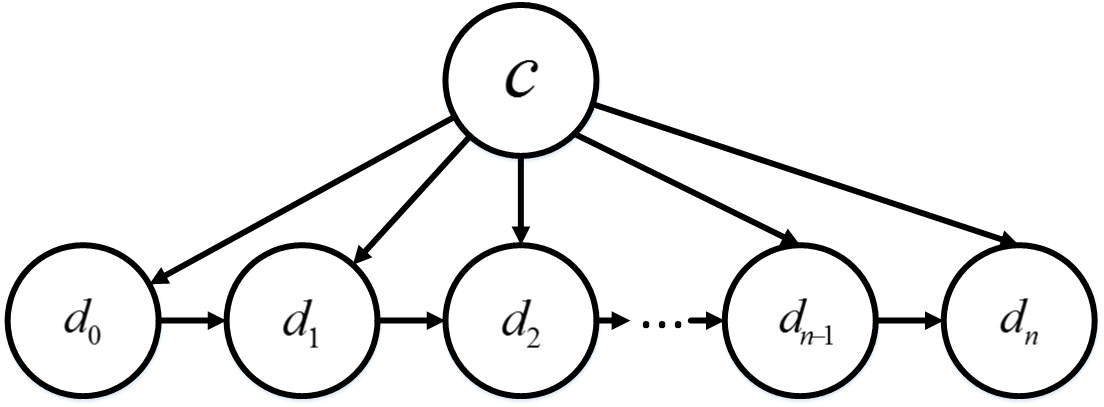
\includegraphics[width=150mm]{tracking/Trajectory}
		\caption{Графическая модель произвольной траектории. $c$ "--- тип траектории.}
		\label{sec::tracking::fig::trajectory}
	\end{center}
\end{figure}

Правдоподобие для каждой траектории $T$ определяется по следующей формуле:
\begin{equation}
	p(T={d_0, d_1, d_2, \dots, d_{n-1}, d_n}|c) = p(d_0|c)\prod_ip(d_i|d_{i-1}, c)
	\label{sec::tracking::eq::track_prob}
\end{equation}

Из формулы \eqref{sec::tracking::eq::track_prob} следует, что для определения правдоподобия траектории необходимо определить $p(d_0 |c)$ "--- вероятность наблюдения первого треклета траектории и  $p(d_i|d_{i-1}, c)$ "--- вероятность перехода от одного треклета к следующему.

В настоящей работе, как и в статье \cite{benfold2011stable}, каждый треклет предлагается описывать его размером s, положением x на кадре, и оценкой движения m. Чтобы поведение алгоритма не зависело от масштаба, его положение x оценивается не в пикселях, а в размерах треклета. Добавление оценки движения m в информацию о треклете обусловлена необходимостью разделять траектории ложных обнаружений и людей. Из предположения о неподвижности ложных обнаружений вытекает, что для решения описанной проблемы оценкой движения может служить гистограмма абсолютных значений скорости. Оценки для скорости треклета были получены на этапе его построения.

Таким образом, вероятность наблюдения первого треклета траектории и вероятность перехода от одного треклета к следующему факторизуются следующим образом:
\begin{align}
	p(d 0 |c) &= p(s 0 )p(x 0 )p(m 0 |c) \\
	p(d_i|d_{i-1}, c) &= p(s_i | s_{i-1})p(x_i|x_{i-1}, c)p(m_i|c)
\end{align}

Размер первого треклета не может быть оценен через размеры других треклетов траектории. Поэтому в статье \cite{benfold2011stable} предлагается использовать предположение, что логарифм размера первого треклета имеет нормальное распределение:
\begin{equation}
	\ln s_0 \sim N(\mu_p, \sigma_p^2)
\end{equation}

Размеры следующих треклетов траектории существенно зависят от размеров предыдущих.
\begin{equation}
	\ln{\frac{s_i}{s_i{i-1}}}\bigg\rvert c_{ped} \sim N(0, \delta_t, \sigma_{s, p}^2),
\end{equation}
где $\delta_t$ "--- разница во времени между кадрами, на которых были сделаны соответствующие обнаружения.

Аналогично размер первого треклета не может быть оценен через размеры других треклетов траектории. Для использования априорных предпочтений о положении объекта необходима семантическая информация о наблюдаемой сцене: положение дорог, неба, домов и т.д. Извлечение такой семантической информации требует сложного анализа сцены и большого количества вычислительных ресурсов \cite{fulkerson2009class}. Поэтому для первых треклетов траектории требуется только близость к областям входа в сцену:
\begin{equation}
 	p_1(x_0) = N(\rho(x_0, enter)|0, \sigma_d^2),
 	\label{sec::tracking::eq::border_x}
\end{equation}
где $\rho(x_0, enter)$ "--- расстояние от положения первого треклета $x_0$ до ближайшей области входа в сцену. Поиск областей входа в сцену происходит во время сопровождения.

В некоторых случаях объект может быть обнаружен только через некоторое время после того, как он появился в сцене. Это происходит из-за невозможности часто производить поиск объектов и ошибок детекторов. Для корректной обработки таких траекторий строится дополнительное априорное предположение о равномерном распределении первого треклета траектории
на изображении:
\begin{equation}
	p_2(x_0)= \frac{x_0^2}{\alpha},
	\label{sec::tracking::eq::uniform_x}
\end{equation}
где $\alpha$ "--- размер изображения в пикселях.

В результате априорное распределение первого треклета траектории представляется в виде смеси распределений \eqref{sec::tracking::eq::border_x} и \eqref{sec::tracking::eq::uniform_x}:
\begin{equation}
	p(x_0) = \frac{p_1(x_0) + p_2(x_0)}{2}
\end{equation}

Как описано выше, в настоящей работе предполагается, что ложные обнаружения не изменяют своего положения. Таким образом, изменение положения треклетов ложных обнаружений происходит лишь вследствие случайного шума:
\begin{equation}
	x_i\bigg\rvert x_{i-1}, c_{fp} \sim N(x_{i-1}, 2\Sigma_d)
\end{equation}

Положение треклета траектории человека зависит от положения предыдущего треклета более сложным образом. Для упрощения вычислений в настоящей работе, как и в статье \cite{benfold2011stable}, делается предположение о равномерности движения человека между
обнаружениями. Сначала предлагается сделать прогноз о положении следующего треклета на основе наиболее надежной оценки скорости треклета $d_{i-1}$:
\begin{equation}
	\begin{aligned}
		x_p^{i-1} &= x_{i-1} + \delta_t v_p \\
		\Sigma_p &= \delta_t\Sigma_v
	\end{aligned}
\end{equation}

Оценка скорости v p получается из результатов сопровождения обнаружения на кадрах сразу следующим за текущим и непосредственно ему предшествующим. Данная оценка считается наиболее надежной, поскольку вероятность ошибки алгоритма визуального сопровождения на этих кадрах наименьшая. С другой стороны, полученный прогноз может быть неточным из-за неравномерности движения человека. Поэтому предлагается уточнять полученное положение за счет имеющихся оценок скорости.

Оценки скорости, полученные при построении треклетов, позволяют уточнить положение следующего треклета. В связи с этим для каждой оценки скорости $y_{i-1}$ треклета $d_{i-1}$ предлагается, как и в статье \cite{benfold2011stable}, вычислять апостериорное распределение на положение следующего треклета, при помощи уточнения построенного прогноза:
\begin{align}
	x_y^{i-1}&=x_p^{i-1} + \Delta x_y \\
	x_p^{y_{i-1}}&= x_{i-1} + \delta_t y_{i-1} \\
	\Delta x_y &= \Sigma_p (\Sigma_p + \delta_t \Sigma_{local})^{-1}(x_p^{y_{i-1}} - x_p^{i-1}) \\
	\Sigma_y &= (I - \Sigma_p(\Sigma_p + \delta_t \Sigma_{local})^{-1})\Sigma_p,
\end{align}
где $\Sigma_local$ отображает скорость, с которой алгоритм визуального сопровождения, используемый при построении треклетов, накапливает случайную ошибку, $\delta_t$ "--- разница между временными метками треклетов $d_{i-1}$ и $d_i$. Заметим, что уточнение происходит так же, как и в шаге обновления в фильтре Калмана~\cite{kalman1960new}.

Стоит отметить, что такой прогноз положения, хотя и является более точным, менее надежен из-за увеличения с каждым кадром вероятности потерять сопровождаемого человека алгоритмом визуального сопровождения. В связи с этим в статье \cite{benfold2011stable} предлагается определить распределение положения следующего треклета с помощью смеси нормальных распределений:
\begin{equation}
p(x_i|x_{i-1}, Y_{i-1}, c_{ped}) = \frac{\alpha^{\sigma_t}}{\left|Y_{i-1}\right|}\Sigma_{y\in Y_{i-1}}N(x_y^{i-1}, \Sigma_y + 2\Sigma_d) + (1+\alpha^{\sigma_t})N(x_p^{i-1}, \Sigma_p + 2\Sigma_d)
\end{equation}

Параметр $\alpha$ соответствует вероятности потерять сопровождаемого человека используемым алгоритмом визуального сопровождения. $(1-\alpha)\delta_t$ "--- вероятность того, что сопровождаемый человек не был потерян в течении $\delta_t$ секунд.

В настоящей работе было замечено, что использование оценок скорости не только треклета $d_{i-1}$ , но и треклета $d_i$ улучшает качество сопровождения. Поэтому, распределение положения треклета $d_i$ предлагается определить следующим образом:
\begin{equation}
	p(x_i |x_{i-1}, Y_i, Y_{i-1}, c_{ped}) = \beta p(x_i|x_{i-1}, Y_i, c_{ped}) + (1 - \beta) p(x_i|x_{i-1}, Y_{i-1}, c_{ped}),
\end{equation}
где $Y_i$ и $Y_{i-1}$ "--- множества используемых оценок скорости треклетов $d_{i-1}$ и $d_i$ соответственно. Параметр $\beta$ указывает какой оценке дается большее предпочтение:
\begin{equation}
	\beta=\frac{\left|Y_{i-1} + 1\right|}{\left|Y_{i-1}\right| + \left|Y_i\right| + 2}
\end{equation}

В отличие от статьи \cite{benfold2011stable}, где предлагается использовать все оценки скорости треклета, в данной работе используются лишь те оценки скорости, которые получены из положения сопровождаемого человека в момент обнаружения и его положений между обнаружениями треклетов $d_i$ и $d_{i-1}$. Благодаря этому, во-первых, используются только самые надежные оценки скорости, во-вторых, используется предположение равномерности движения человека только между соседними обнаружениями.

Для завершения описания модели движения траектории необходимо задать распределение оценку движения $m$. Оценка движения необходима только для отделения траекторий человека от траекторий ложных обнаружений, у которых, как предполагается, движение отсутствует. В связи с этим, движение, как и в статье \cite{benfold2011stable}, моделируется гистограммой из 4 корзин. Границы корзин моделируют движение в размере $frac{1}{8}, frac{1}{4}$ и $\frac{1}{2}$ размера треклета. Предполагается, что гистограмма принадлежит одному из двух мультиномиальных распределений, зависящему только от типа траектории:
\begin{align}
m_i |c_{ped} &\sim \mathop{Mult}(m_{ped}) \\
m_i |c_{fp} &\sim \mathop{Mult}(m_{fp})
\end{align}

Как было описано выше, задача ассоциирования треклетов сводится к задаче построения оптимального множества траекторий, включающего все наблюдаемые треклеты $D$. Так же необходимо определить тип c каждой траектории. Тогда гипотезу можно определить следующим образом $H = \left\{\left(T i , c i \right)\right\}^n_{i=1}$. В силу формулы условной вероятности задача поиска оптимальной гипотезы \eqref{sec::tracking::opt_hyp} эквивалентна следующей задаче:
\begin{equation}
H^* = \argmax_H p(D|H)p(H)
\end{equation}

Определим априорное распределение гипотезы следующим образом:
\begin{equation}
	p(H) = J!\prod_{T_j \in H}\left(\frac{\left|T_j\right|}{D}\right)^{\left|T_j\right|}p(c_j),
\end{equation}
где $J$ "--- количество траекторий в гипотезе $H$, $p(c_j)$ "--- априорная вероятность типа траектории. Так же в силу независимости траекторий правдоподобие представляется в
следующем виде:
\begin{equation}
	P(D|H) = p(T_1, T2, ..., T_J|H) = \prod_{t_j\in H}p(T_j|c_j)
\end{equation}
Здесь правдоподобие каждой траектории $p(T_j|c_j)$ определяется согласно формуле \eqref{sec::tracking::eq::track_prob}.

Алгоритм ассоциирования

Как было описано выше, для ассоциирования треклетов необходимо найти гипотезу $H$:
\begin{equation}
	H^* = \argmax_H p(D|H)p(H)
\end{equation}

Заметим, что сложность нахождения оптимальной гипотезы растет с длительностью сопровождения в видеопоследовательности, поскольку увеличивается количество обрабатываемых треклетов. В связи с этим в настоящей работе, как и в статье \cite{benfold2011stable}, предлагается обрабатывать те треклеты, которые попали в заранее заданное скользящее окно. Данноескользящее окно включает кадры с временной меткой из отрезка $(t - \delta, t]$, где $t$ "--- временная метка кадра, обрабатываемого в настоящий момент. В каждый момент времени только для этого множества треклетов предлагается строить гипотезу разбиения их на траектории.

К сожалению, нет эффективного алгоритма для получения гипотезы, на которой достигается глобальный максимум функции распределения. Поэтому предлагается использовать метод приближенного вывода "--- алгоритм MCMC DA. Данный алгоритм предполагает построение выборки гипотез из распределения $p(H, D)$ по схеме Марковских цепей. После этого гипотеза с наибольшей апостериорной вероятностью принимается в качестве приближения оптимальной гипотезы.

Рис. 5. Примеры типов проводимых изменений гипотез. Слева показан пример обмена. На рисунке справа показан пример переключения.

Для построения выборки из распределения гипотез используется алгоритм Метрополиса-Гастингса~\cite{oh2004markov} (алгоритм 1).

В качестве инициализации используется гипотеза, полученная после обработки предыдущего кадра. Треклеты, вышедшие за пределы скользящего окна, исключаются из траекторий.Новые треклетыдобавляются к траекториям с помощью жадного алгоритма. Таким образом, удается получить хорошее начальное приближение для алгоритма Метрополиса-Гастингса.

Новая гипотеза $\hat{H}$ получается, как и в статье \cite{benfold2011stable}, из гипотезы $H_i$, построенной на предыдущем шаге, посредством изменений трех типов:
\begin{itemize}
	\item Обмен;
	\item Переключение;
	\item Изменение типа.
\end{itemize}
При обмене случайно выбираются траектории $T_1$ и $T_2$ и треклет $d$ первой из них. После этого траектория $T_1$ отдает треклет $d$ траектории $T_2$. Если траектория $T_2$ содержала треклет с той же временной меткой, то происходит обмен этими конфликтующими треклетами. В противном случае траектория $T_1$ отдает выбранный треклет (рисунок 5).

При переключении случайно выбираются 2 траектории $T_1$ и $T_2$ и произвольный момент времени $t$ внутри скользящего окна. Траектории обмениваются всеми треклетами с временными метками больше $t$ (рисунок 5).

При изменении типа случайным образом выбирается траектория $T$. После этого происходит изменение её типа с <<человек>> на <<ложное обнаружение>> или наоборот.

Важно отметить, что в изменениях первого и второго типов при выборе траекторий используются дополнительные пустые траектории с типами <<человек>> и <<ложное обнаружение>> соответственно. Это позволяет создавать новые, до этого момента не существовавшие траектории. Так же если во время одного из описанных выше изменений, траектория становится пустой, то есть не содержащей ни одного треклета, то она удаляется из гипотезы $\hat{H}$.


Таким образом, благодаря описанным выше типам изменения гипотез, можно за конечное число шагов получить любую допустимую гипотезу.

В алгоритме Метрополиса-Гастингса вероятность принять построенную гипотезу вычисляется по следующей формуле:
\begin{equation}
	p(H_{i+1}|\hat{H}) = \min \left(\frac{p(\hat{H}, D)q(H_i|\hat{H})}{p(H_i, D)q(\hat{H}|H_i)}, 1\right)
\end{equation}

Здесь $q(H_i|\hat{H})$ и $q(\hat{H}|H_i)$ "---вероятности перейти от гипотезы $\hat{H}$ к $H_i$ и от $H_i$ к $\hat{H}$ соответственно. Заметим, что, так как тип выполняемого изменения, треклет и временная метка выбираются каждый раз из равномерного распределения, то во многих ситуациях вероятности описанных переходов равны. Исключениями являются переходы, при которых изменяется количество траекторий гипотезы. Это может происходить из-за удаления или создания новых гипотез при обмене или переключении.

Так же важно отметить, что при обмене и переключении между траекториями одного типа нет необходимости пересчитывать правдоподобие обеих траекторий целиком, так как для большинства треклетов траекторий значения соответствующих вероятностей не изменяются. Так при обмене необходимо пересчитывать значения вероятностей не более чем для четырех треклетов, а при переключении между траекториями одного типа "--- не более чем для двух. Благодаря, этому появляется возможность осуществлять значительное число итерация алгоритма Метрополиса-Гастингса. Так в реализации предлагаемого алгоритма для каждого обрабатываемого кадра проводилось 2000 итераций.

Восстановление положения

На последнем шаге предлагаемого алгоритма происходит определение положения каждого человека на каждом кадре видеопоследовательности. Для этого необходимо преобразовать оптимальную гипотезу во множество прямоугольников, ограничивающих изображения людей. В алгоритме проводится восстановление положения людей для кадра, соответствующего задержке в видеопоследовательности, равной двум секундам. Это позволяет учитывать информацию о движении человека до и после этого кадра. Как было описано выше, не все траектории гипотезы описывают движение людей. Также траектории людей, содержащие малое количество треклетов часто являются ошибочными или содержат ложные обнаружения. Таким образом, предлагается проводить постобработку построенной гипотезы.

\begin{table}[h]
	\caption{Результаты тестирования на выборке TownCentre}\label{sec::tracking:tab::comparison} \centering
	\begin{tabular}{|c|c|c|}
		\hline
		Результаты тестирования & MOTA & MOTP\\
		\hline \hline
		Benfold и~др. \cite{benfold2011stable} & 0.454 & 0.508 \\ \hline
		Кросс-корреляция шаблонов & 0.507 & 0.524 \\ \hline
		<<Стая точек>> & 0.519 & 0.525 \\ \hline
		<<Стая точек>> + регионы входа/выхода & 0.54 & 0.522 \\ \hline
	\end{tabular}
\end{table}

Рассмотрим сначала, как происходит восстановление положения человека на ключевом кадре, где он был обнаружен. Этот этап необходим, так как используемый детектор позволяет локализовать только изображение головы человека. Для решения этой задачи на этапе фильтрации обнаружений определяется не только их размер, но и положение людей на плоскости земли. Проекция каждой такой точки на плоскость изображения соответствует нижней границе прямоугольника, ограничивающего изображение человека. Его верхняя граница совпадает с верхней границей прямоугольника, ограничивающего изображение найденной детектором головы.

Для восстановления положения человека между ключевыми кадрами используется предположение о равномерности движения человека между обнаружениями. Поэтому положение человека на промежуточных кадрах определяется с помощью линейной интерполяции.

Поиск областей входа в сцену

\begin{figure}[t]
	\begin{center}
		\begin{tabular}{cc}
		 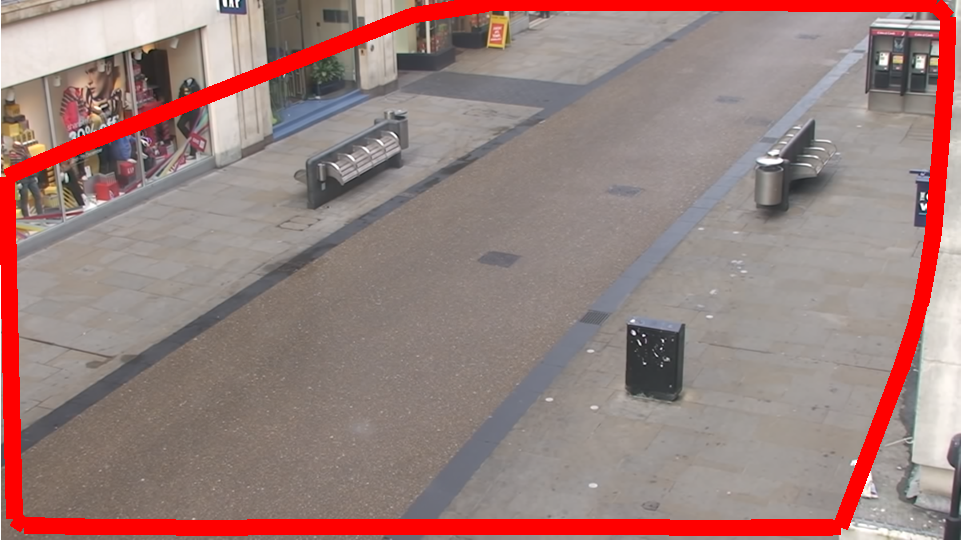
\includegraphics[width=75mm]{tracking/border} & 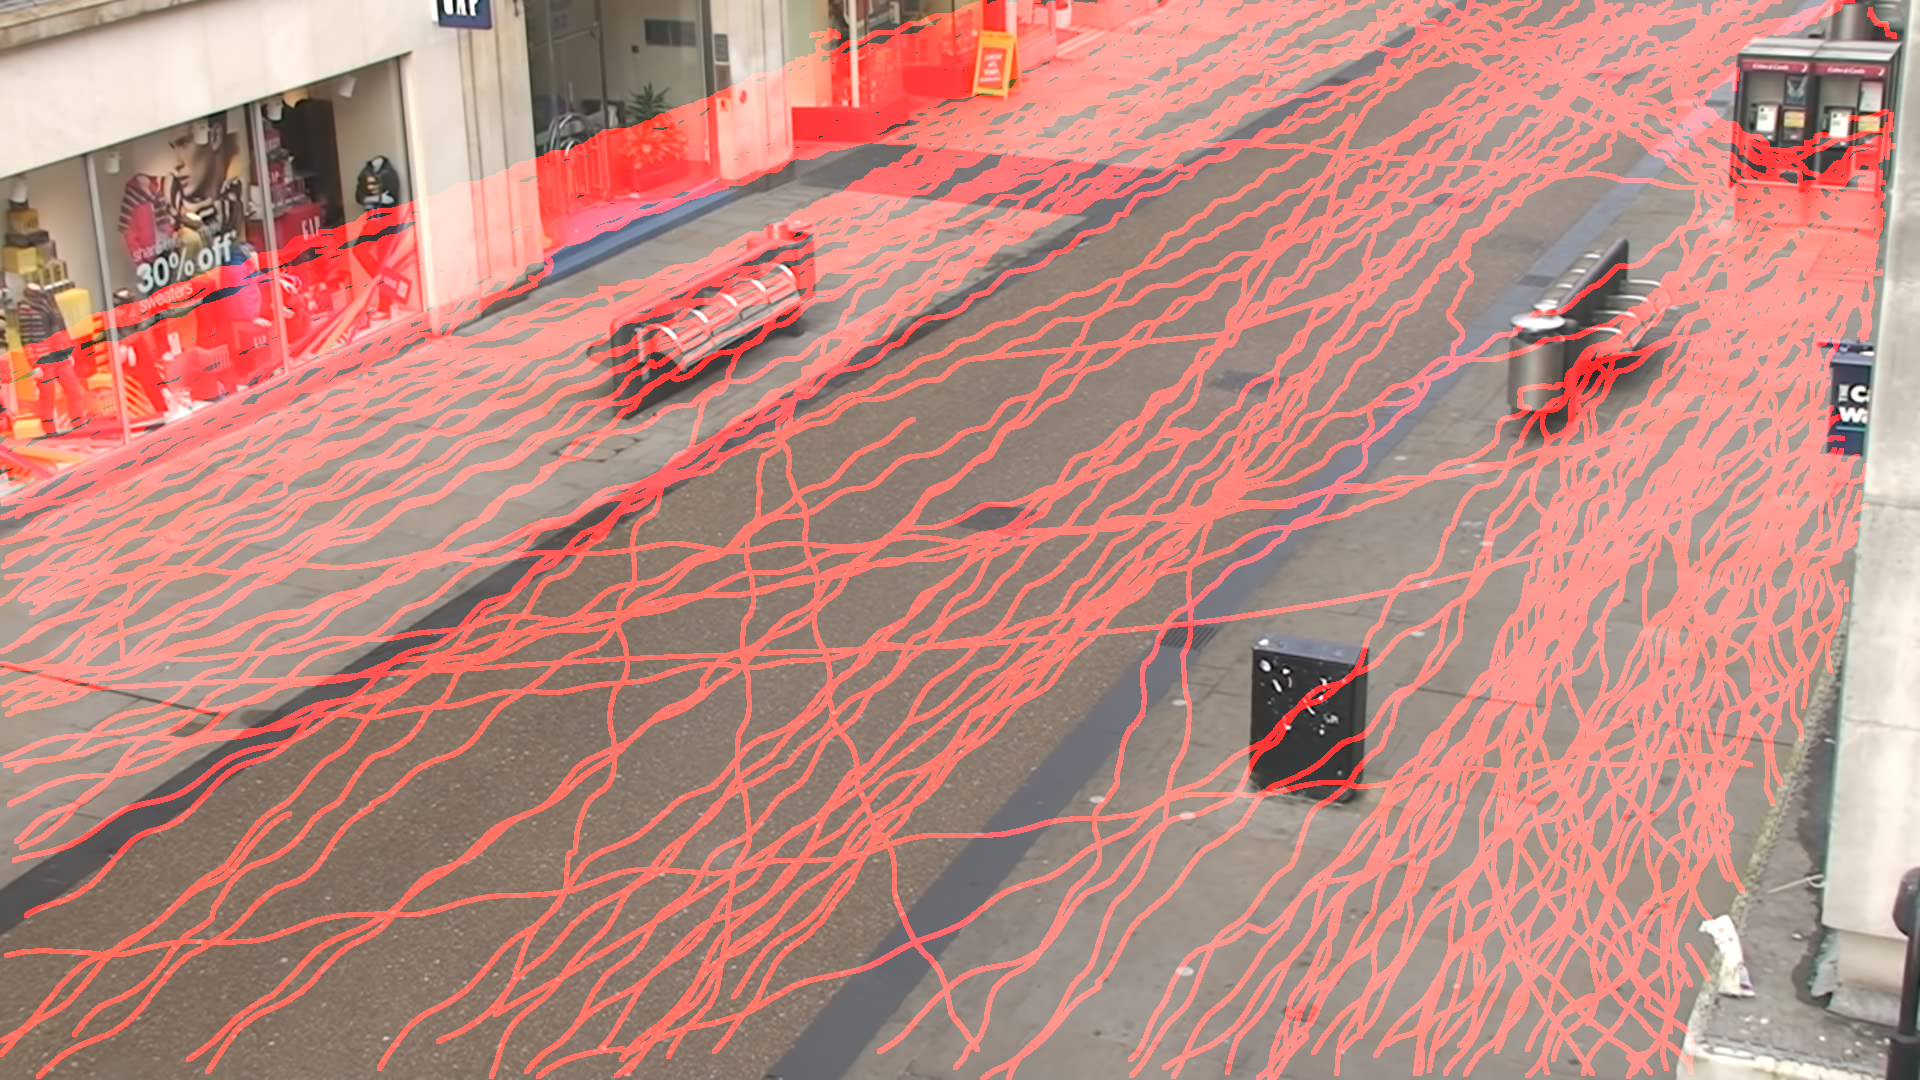
\includegraphics[width=75mm]{tracking/trajectories} \\
		(а) & (б)
		\end{tabular}
		\caption{Поиск областей входа в сцену. (а) найденная область входа в сцену; (б) визуализация траекторий экспертной разметки}
		\label{sec::tracking::fig::border}
	\end{center}
\end{figure}

Как было сказано ранее, поиск областей входа в сцену осуществляется автоматически. В настоящей работе предполагается, что данные области образуют выпуклый многоугольник на изображении (рисунок~\ref{sec::tracking::fig::border}~(а)). Тогда расстояние до области входа в сцену можно определить, как расстояние до границы этого многоугольника. В качестве такого многоугольника выбирается выпуклая оболочка положений первых и последних треклетов устойчивых траекторий. Такое представление области входа в сцену позволяет проводить его обновление каждый раз после ассоциирования треклетов с траекториями. Обозначим через $d_0^j$, $d_{n_j}^j$ первый и последний треклет траектории $T_j$ , а через $x_0$ , $x_{n_j}$ их положения. Тогда обновление областей входа в сцену можно осуществлять так, как описано в алгоритме 2.

Среди недостатков такого подхода можно выделить неустойчивость к выбросам. Если область входа в сцену была ошибочно увеличена, то она никогда не сможет быть уменьшена в дальнейшем. В связи с этим необходимо учитывать только надёжные траектории. В этой работе надёжными я считал траектории, содержащие не менее 5 треклетов человека. Можно заметить, что построенная область входа в сцену соответствует границе области, содержащей траектории экспертной разметки (рис.~\ref{sec::tracking::fig::border}~(б))

Другим недостатком такого подхода является учет препятствий на границе сцены в качестве точек входа. Примером таких препятствий может служить стена здания изображенная на рисунке~\ref{sec::tracking::fig::border}~(а). 

Полученные результаты

Предложенный алгоритм тестировался на открытой базе TownCentre \cite{benfold2011stable}. Она содержит видеопоследовательность высокого разрешения (1920x1080/25fps), снятую статичной камерой. Так же присутствует экспертная разметка, которая состоит из 71500 вручную размеченных положений голов людей. В среднем на каждом кадре присутствуют 16 человек.

Для оценки качества сопровождения использовались критерии MOTA и MOTP \cite{bernardin2008evaluating}. MOTA описывает качество построения траекторий людей, а MOTP "--- точность определения положения людей на кадрах видеопоследовательности. В связи с этим наиболее информативным является критерий MOTA. Значение критерия MOTA не превосходят 1, а значения критерия MOTP неотрицательны. Увеличение значения критерия MOTA свидетельствует об улучшении качества построенных траекторий людей, в то время как уменьшение значения MOTP говорит о повышении точности определения положения людей.

Результаты тестирования представлены в таблице \ref{sec::tracking:tab::comparison}. Алгоритмы, представленные во второй и третьей строках таблицы, различаются способом построения треклетов. Использование алгоритма <<Стая точек>> дает лучшие результаты на тестовой базе TownCentre, но качество сопровождения голов данным алгоритмом существенно зависит изображения головы человека. На слабо текстурированных изображениях голов не всегда удается найти достаточное количество уголков. В такой ситуации алгоритм сопровождения на основе кросс-корреляции шаблонов более устойчив к потере головы человека. Поэтому при дальнейшем развитии работы предлагается выбирать алгоритм визуального сопровождения в зависимости качества изображения головы человека.

В последней строке представлены результаты работы предлагаемого алгоритма при использовании алгоритма <<Стая точек>> и учёте областей входа в сцену.

Анализ алгоритма

Как было указано выше, предлагаемый метод сопровождения представляет конвейер из последовательно применяемых алгоритмов (рисунок 1). Поэтому важным является вопрос о том, какая часть данного конвейера является самой слабой частью метода. Одним из наиболее эффективных способов ответа на этот вопрос является метод, основанный на последовательном
исключении первых этапов конвейера из алгоритма.

Данный метод заключается в последовательной замене результатов, получаемых на начальных этапах конвейера, на результаты экспертной разметки. Это позволяет оценить, какой вклад в общую ошибку дает каждый этап.

Результаты анализа представлены в таблице \ref{sec::tracking:tab::ceiling_analysis}. В первом столбце указан этап конвейера, который был заменен экспертной разметкой. Исключение составляет только первая строка, где приведены результаты работы конвейера целиком. Во втором и третьем столбце указаны значения критерием MOTA и MOTP соответственно. Из результатов анализа следует, что улучшение алгоритма построения траекторий может дать наибольшее увеличение надежности сопровождения (около 0,28 с 0,629 до 0,916). Также анализ показал, что предположение о линейности движения людей между обнаружениями является очень грубым приближением поскольку замена алгоритма восстановления положения людей на промежуточных кадрах на их положение в экспертной разметке увеличивает надежность сопровождения более, чем на 0,07. Также об этом свидетельствует повышение значения критерия MOTP при использовании траекторий, полученных из экспертной разметки. Данное повышение означает, что алгоритм построения траекторий совершал больше всего ошибок в случаях нелинейного движения.

\begin{table}[h]
	\caption{Анализ этапов конвейера} \label{sec::tracking:tab::ceiling_analysis} \centering
	\begin{tabular}{|c|c|c|}
		\hline
		 & MOTA & MOTP\\
		\hline \hline
		Весь конвейер & 0.54 & 0.522 \\ \hline
		Поиск людей & 0.562 & 0.143 \\ \hline
		Построение треклетов & 0.629 & 0.145 \\ \hline
		Построение траекторий & 0.916 & 0.383 \\ \hline
		Восстановление положения & 0.988 & 0.083 \\ \hline
	\end{tabular}
\end{table}

Анализ показал, что используемый алгоритм поиска людей позволяет определить положение для достаточного для надежного сопровождения количества людей, но при этом точность локализации оказывается низкой. Стоит отдельно отметить почему не удается получить идеальных результатов даже в случае, если заменить последний этап конвейера на результаты экспертной разметки. В предлагаемом алгоритме поиск объектов осуществлялся 5 раз в секунду, то есть лишь на одном из пяти кадров. Также для положения сопровождаемых людей не проводилась экстраполяция вне сегмента между первым и последним обнаружениями. Это приводит к тому, что длительность сопровождения человека в  экспертной разметке во многих случаях превышает длительность сопровождения предлагаемым алгоритмом. На точность локализации людей на изображении повлияло предположение о равенстве ширины и высоты прямоугольника, ограничивающего изображение головы человека. Вклад этого предположения отражен в значении критерия MOTP последней строке.

\section{Модель наблюдаемых данных}
\subsection{Модель детектора}
\subsection{Модель движения}
\section{Предложенный метод}
\subsection{Базовый метод}
\subsection{Предложенный метод оценки скорости}
\subsection{Определение областей входа/выхода}
\section{Экспериментальная оценка}
